
\documentclass[12pt,a4paper]{article}
\usepackage{amsfonts,amsmath,amssymb,graphicx}
\usepackage[francais]{babel}
\usepackage[latin1]{inputenc}
\usepackage{answers}
\usepackage{a4wide,commeunjeustyle} 

%---- Dimensions des marges ---
\setlength{\paperwidth}{21cm} 
\setlength{\paperheight}{29.7cm}
\setlength{\evensidemargin}{0cm}
\setlength{\oddsidemargin}{0cm} 
\setlength{\topmargin}{-2.5cm}
\setlength{\headsep}{0.7cm} 
\setlength{\headheight}{1cm}
\setlength{\textheight}{25cm} 
\setlength{\textwidth}{17cm}




%---- Structure Exercice -----
\newtheorem{Exc}{Exercice}
\Newassociation{correction}{Soln}{mycor}
\Newassociation{indication}{Indi}{myind}
%\newcommand{\precorrection}{~{\bf \footnotesize [Exercice corrig\'e]}}
%\newcommand{\preindication}{~{\bf \footnotesize [Indication]}}
\renewcommand{\Solnlabel}[1]{\bf \emph{Correction #1}}
\renewcommand{\Indilabel}[1]{\bf \emph{Indication #1}}

\def\exo#1{\futurelet\testchar\MaybeOptArgmyexoo}
\def\MaybeOptArgmyexoo{\ifx[\testchar \let\next\OptArgmyexoo
                        \else \let\next\NoOptArgmyexoo \fi \next}
\def\OptArgmyexoo[#1]{\begin{Exc}[#1]\normalfont}
\def\NoOptArgmyexoo{\begin{Exc}\normalfont}

\newcommand{\finexo}{\end{Exc}}
\newcommand{\flag}[1]{}

\newtheorem{question}{Question}



%---- Style de l'entete -----                     % -> � personnaliser <-
\setlength{\parindent}{0cm}
\newcommand{\entete}[1]
{
{\noindent
  \textsf{Feuille d'exercices}            % Universit�
}
\hrule
\hrule
\begin{center} 
\impo{\textsf{\Large 
     D�nombrement     % TITRE
}}
\end{center}
\hrule
}


\begin{document}

%--- Gestion des corrections ---
 \Opensolutionfile{mycor}[ficcorex]
 \Opensolutionfile{myind}[ficind]
 \entete{\'Enonc�s}
\exo{ 0402 , tariel, 01/11/2017, 1-2, {}}[*, Anagramme]
D�nombrer les anagrammes des mots suivants : MATHS, RIRE.
   
\begin{correction}
Un anagramme du mot MATHS correspond � une permutation des lettres, soit  5! fa�ons.\\
Pour le second mot, voici deux r�ponses possibles : 
\begin{enumerate}
\item en utilisant le principe de d�composition, on place d'abord la lettre R, soit 2 lettres parmi 4, d'o� 4!/(2!2!) combinaisons, puis la lettre I (il reste 2 places), soit 2 combinaisons , et enfin la lettre E (il reste 1 place), soit 1 combinaison. En multipliant ces combinaisons, on obtient  4!/2! combinaisons.
\item R est pr�sent deux fois et si on permute cette lettre, on trouve le m�me mot.
On doit donc diviser le nombre total de permutations par le nombres de permutations entre lettres identiques, d'o�  4!/2! combinaisons.
\end{enumerate}
\end{correction}

\finexo
\exo{ 0402 , tariel, 01/11/2017, 1-2, {}}[*, Code secret]
Combien y a-t-il de codes secrets de $5$ chiffres o� $0$ figure une fois et une seule~?

\begin{correction}
D'abord, on place le $0$ soit au chiffre des unit�s (****0), soit au chiffre des dizaines (***0*), soit au chiffre des centaines (**0**), soit au chiffre des milliers (*0***) soit au chiffre des dizaines de milliers (0****). Puis on remplace chaque * par un chiffre entre 1 et 9.   D'apr�s le principe de d�composition, on a :~$5.9.9.9.9=4.9^4$.
\end{correction}

\finexo
\exo{ 0402 , tariel, 01/11/2017, 1-2, {}}[*, Poker]
Lors d'une partie de poker, un joueur re�oit 5 cartes d'un jeu de 52 cartes ; ce qui constitue une main.\\
\begin{enumerate}
\item Combien y a-t-il de mains possible ? 
\item Combien y a-t-il de mains possible avec un carr� ? ex. 1$\clubsuit$ 1$\blacklozenge$ 1$\heartsuit$ 1$\spadesuit$ V $\heartsuit$
\item Combien y a-t-il de mains avec un full ? ex. R$\clubsuit$ R$\blacklozenge$ 8$\heartsuit$ 8$\spadesuit$ 8$\clubsuit$
\item  Combien y a-t-il de mains avec une double paire ? ex. D$\clubsuit$ D$\blacklozenge$ 8$\heartsuit$ 8$\clubsuit$ R$\spadesuit$
\item  Combien y a-t-il de mains avec un brelan ? ex. V $\clubsuit$ V $\blacklozenge$ V $\heartsuit$ 1$\spadesuit$ 9$\clubsuit$
\item  Combien y a-t-il de mains avec une paire ? ex. D$\clubsuit$ D$\blacklozenge$ 7$\heartsuit$ 9$\spadesuit$ V $\clubsuit$
\item  Combien y a-t-il de mains avec une quinte flush ? ex. 7$\clubsuit$ 8$\clubsuit$ 9$\clubsuit$ 10$\clubsuit$ V $\clubsuit$
\item  Combien y a-t-il de mains avec une suite ? ex. 8$\clubsuit$ 9$\blacklozenge$ 10$\heartsuit$ V $\spadesuit$ D$\blacklozenge$
\item  Combien y a-t-il de mains avec une couleur ? ex. 1$\heartsuit$ 7$\heartsuit$ 10$\heartsuit$ D$\heartsuit$ R$\heartsuit$
\end{enumerate}
\begin{correction}
\begin{enumerate}
\item Une main correspond � un tirage sans remise et sans ordre. Donc le nombre de mains est $\begin{pmatrix}52\\5\end{pmatrix}$
\item \textit{nombre de mains avec un carr� :} d'apr�s le principe de d�composition,  on a  
$$\overbrace{\overbrace{\begin{pmatrix}13\\1\end{pmatrix}}^
{\begin{subarray}{l}\text{1 hauteur}\\
    \text{parmi 13}\end{subarray}}
\times    \overbrace{\begin{pmatrix}4\\4\end{pmatrix}}^{\begin{subarray}{l}\text{4 cartes parmi}\\
    \text{les 4 de la hauteur}\end{subarray}}}^{\text{carr�}}
\times     \overbrace{\begin{pmatrix}48\\1\end{pmatrix}}^{\text{carte restante}}=624$$
\item  \textit{nombre de mains avec un full :} d'apr�s le principe de d�composition,  on a  
$$
\overbrace{\overbrace{\begin{pmatrix}13\\1\end{pmatrix}}^
{\begin{subarray}{l}\text{1 hauteur}\\
    \text{parmi 13}\end{subarray}}
\times    \overbrace{\begin{pmatrix}4\\3\end{pmatrix}}^{\begin{subarray}{l}\text{3 cartes parmi}\\
    \text{les 4 de la hauteur}\end{subarray}}}^{\text{brelan}}
\times\overbrace{\overbrace{\begin{pmatrix}12\\1\end{pmatrix}}^
{\begin{subarray}{l}\text{1 hauteur}\\
    \text{parmi 12}\end{subarray}}
\times    \overbrace{\begin{pmatrix}4\\2\end{pmatrix}}^{\begin{subarray}{l}\text{2 cartes parmi}\\
    \text{les 4 de la hauteur}\end{subarray}}}^{\text{pair}}=3744
    $$
\item \textit{nombre de mains avec une double paire :} d'apr�s le principe de d�composition,  on a  
$$
\overbrace{\overbrace{\begin{pmatrix}13\\2\end{pmatrix}}^
{\begin{subarray}{l}\text{2 hauteurs}\\
    \text{parmi 13}\end{subarray}}
\times    \overbrace{\begin{pmatrix}4\\2\end{pmatrix}}^{\begin{subarray}{l}\text{2 cartes parmi}\\
    \text{les 4 d'une pair}\end{subarray}}
\times    \overbrace{\begin{pmatrix}4\\2\end{pmatrix}}^{\begin{subarray}{l}\text{2 cartes parmi}\\
    \text{les 4 de l'autre pair}\end{subarray}}}^{\text{double pairs}}
    \times    \overbrace{\begin{pmatrix}24\\1\end{pmatrix}}^{\text{carte restante}}=3744
$$
Attention, il faut choisir deux paires diff�rentes sinon
c'est un carr�. De plus, le nombre de mains n'est pas 
$$
\overbrace{\overbrace{\begin{pmatrix}13\\1\end{pmatrix}}^
{\begin{subarray}{l}\text{1 hauteur}\\
    \text{parmi 13}\end{subarray}}
\times    \overbrace{\begin{pmatrix}4\\2\end{pmatrix}}^{\begin{subarray}{l}\text{2 cartes parmi}\\
    \text{les 4 de la hauteur}\end{subarray}}}^{\text{pair}}
\times\overbrace{\overbrace{\begin{pmatrix}12\\1\end{pmatrix}}^
{\begin{subarray}{l}\text{1 hauteur}\\
    \text{parmi 12}\end{subarray}}
\times    \overbrace{\begin{pmatrix}4\\2\end{pmatrix}}^{\begin{subarray}{l}\text{2 cartes parmi}\\
    \text{les 4 de la hauteur}\end{subarray}}}^{\text{pair}}
    \times     \overbrace{\begin{pmatrix}44\\1\end{pmatrix}}^{\text{carte restante}}$$
car on met de l'ordre  dans les paires. Par exemple, on compte deux fois la main:\\
 As Tr�fle, As Carreau, Roi Tr�fle, roi Carreau, 7 C\oe ur\\ et\\
  Roi Tr�fle, Roi Carreau, As Tr�fle, As Carreau 7 C\oe ur.  
\item  \textit{nombre de mains avec un brelan :}
 d'apr�s le principe de d�composition,  on a  
$$\overbrace{
\overbrace{\begin{pmatrix}13\\1\end{pmatrix}}^
{\begin{subarray}{l}\text{1 hauteur}\\
    \text{parmi 13}\end{subarray}}
\times    \overbrace{\begin{pmatrix}4\\3\end{pmatrix}}^{\begin{subarray}{l}\text{3 cartes parmi}\\
    \text{les 4}\end{subarray}}}^{\text{brelan}}
\times \overbrace{   \overbrace{\begin{pmatrix}12\\2\end{pmatrix}}^{\begin{subarray}{l}\text{2 hauteurs parmi}\\
    \text{les 12}\end{subarray}}
\times    \overbrace{\begin{pmatrix}4\\1\end{pmatrix}}^{\begin{subarray}{l}\text{1 carte parmi}\\
    \text{les 4}\end{subarray}}
\times    \overbrace{\begin{pmatrix}4\\1\end{pmatrix}}^{\begin{subarray}{l}\text{1 carte parmi}\\
    \text{les 4}\end{subarray}}}^{\text{2 cartes restantes}}
$$
Attention, il faut choisir deux hauteurs diff�rentes sans ordre pour les 2 cartes restantes pour ne pas avoir une pair formant alors un full.
\item \textit{nombre de mains avec une paire :} d'apr�s le principe de d�composition,  on a  
$$\overbrace{
\overbrace{\begin{pmatrix}13\\1\end{pmatrix}}^
{\begin{subarray}{l}\text{1 hauteur}\\
    \text{parmi 13}\end{subarray}}
\times    \overbrace{\begin{pmatrix}4\\2\end{pmatrix}}^{\begin{subarray}{l}\text{2 cartes parmi}\\
    \text{les 4}\end{subarray}}}^{\text{pair}}
\times \overbrace{   \overbrace{\begin{pmatrix}12\\3\end{pmatrix}}^{\begin{subarray}{l}\text{3 hauteurs parmi}\\
    \text{les 12}\end{subarray}}
\times    \overbrace{\begin{pmatrix}4\\1\end{pmatrix}}^{\begin{subarray}{l}\text{1 carte parmi}\\
    \text{les 4}\end{subarray}}
\times    \overbrace{\begin{pmatrix}4\\1\end{pmatrix}}^{\begin{subarray}{l}\text{1 carte parmi}\\
    \text{les 4}\end{subarray}}
 \times    \overbrace{\begin{pmatrix}4\\1\end{pmatrix}}^{\begin{subarray}{l}\text{1 carte parmi}\\
    \text{les 4}\end{subarray}}   
    }^{\text{3 cartes restantes}}
$$
\item \textit{nombre de mains avec une quinte flush :} d'apr�s le principe de d�composition,  on a  
$$
\overbrace{\begin{pmatrix}13\\1\end{pmatrix}}^
{\text{hauteur du d�but de la suite}}
\times
\overbrace{\begin{pmatrix}4\\1\end{pmatrix}}^
{\text{1 couleur}}
=36$$
\item  \textit{nombre de mains avec une suite :} choisir 5 cartes qui se suivent peu importe
leur couleur et retrancher les quintes flush. D'apr�s le principe de d�composition,  on a  
$$\overbrace{\begin{pmatrix}13\\1\end{pmatrix}}^
{\text{hauteur du d�but de la suite}}
\times
\overbrace{\begin{pmatrix}4\\1\end{pmatrix}^5}^
{\text{les couleur}}-36.$$
\item   \textit{nombre de mains avec une couleur :} choisir une couleur puis 5 cartes dans
la couleur et retrancher les quintes flush. D'apr�s le principe de d�composition,  on a  :
$$\overbrace{\begin{pmatrix}4\\1\end{pmatrix}}^
{\text{1 couleur}}
\times
\overbrace{\begin{pmatrix}13\\5\end{pmatrix}}^
{\text{5 cartes dans une couleur}}-36.$$
\end{enumerate}

\end{correction}

\finexo
\exo{ 0402 , tariel, 01/11/2017, 1-2, {}}[*, g�om�trie]
Soit $n$ droites sur un plan non parall�les  et sans  triplet de droites concourantes. Combien peut-on obtenir de triangles au maximum ?
\begin{correction}
Un triangle appartient � trois droites distinctes, soit un tirage sans ordre et sans remises de 3 boules parmi n. Donc on a $\begin{pmatrix}
n\\3
\end{pmatrix}.$
\end{correction}

\finexo
\exo{ 0402 , tariel, 01/11/2017, 1-2, {}}[*, Mousquetaires]
Les trois mousquetaires (donc quatre personnes avec d'Artagnan), ont m�lang� leurs bottes dans le couloir de l'auberge. D'Artagnan se l�ve en premier et prend deux bottes au hasard.
\begin{enumerate}
\item   Combien de possibilit�s s'offrent � lui?
 \item Combien de choix a-t-il tels que les deux bottes forment une paire (une droite et une gauche quelconques)?
\end{enumerate}
\begin{correction}
\begin{enumerate}
\item  2 bottes parmi 8, soit un tirage sans ordre et sans remises de 2 boules parmi 8. Donc on a $\begin{pmatrix}
8\\2
\end{pmatrix}$
\item choisir un mousquetaire et choisir 2 bottes parmi 2. Donc on a 4.
\end{enumerate}
\end{correction}

\finexo
\exo{ 0402 , tariel, 01/11/2017, 1-2, {}}[*, d�mocratie]
On �lit les 2 d�l�gu�s au hasard parmi une classe de 22 �l�ves avec 14 gar�ons/8 filles et 15 responsables et 7 irresponsables
\begin{enumerate}
\item Combien y a-t-il de mani�res de choisir les 2 d�l�gu�s ? 
\item avec la parit� en plus ?
\item avec 2 personnes irresponsables ?
\end{enumerate}

\begin{correction}
\begin{enumerate}
\item  Une �lection correspond � un tirage sans remise et sans ordre. Donc le nombre de mani�res est $\begin{pmatrix}22\\2\end{pmatrix}$
\item parit� = " choisir 1 gar�on  (parmi 14) et choisir 1 fille (parmi 8) ". D'apr�s le principe de d�composition, on a $\begin{pmatrix}14\\1\end{pmatrix}\begin{pmatrix}8\\1\end{pmatrix}$.
\item irresponsables = " choisir 2 irresponsables  parmi 15. Soit $\begin{pmatrix}15\\2\end{pmatrix}$.
\end{enumerate}
\end{correction}

\finexo
\exo{ 0402 , tariel, 01/11/2017, 1-2, {}}[*, google]
Voici le plan d?une ville am�ricaine, G �tant la gare et H un h�tel :
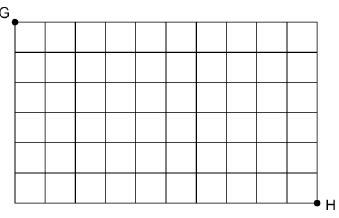
\includegraphics[width=0.25\textwidth]{chemin_court.png}

Chaque bloc est un carr� de 100 m sur 100 m. On cherche d'abord la longueur minimal en se d�pla�ant sur les segments:
\begin{itemize}
\item Comment faut-il se d�placer sur ce quadrillage
si on ne veut pas d�passer la longueur minimale ?
\item  Combien de d�placement pour la longueur minimale ?
\item  Combien de trajets diff�rents y a-t-il
pour aller de la gare � l'h�tel avec cette longueur minimale ?
\end{itemize}
\begin{correction}
\begin{itemize}
\item aller soit � droite soit vers le bas. Si on va gauche, le trajet se rallonge de deux car il faudra compenser en allant une fois � droite. Idem pour vers le haut 
\item 16 d�placements par exemple aller 10 fois � droite puis 6 fois vers le bas
\item On pose B = "vers le bas" et D = "vers la droite". Un exemple de chemin de G � H est le mot
BD...DBB...B o� B est �crit 6 fois et D est �crit 10 fois. Le nombre de chemins cherch� est clairement le
nombre d'anagrammes du mot pr�c�dent. Si on regarde la position du D dans un anagramme, on se ram�ne � un triage sans remise et sans ordre.
Donc le nombre de chemins est 6 parmi 16, soit $\begin{pmatrix}
16\\6
\end{pmatrix}$
\end{itemize}
\end{correction}

\finexo
\exo{ 0402 , tariel, 01/11/2017, 1-2, {}}[*, rangement]
Mr T a 5 livres d'alg�bre, 3 livres de g�om�trie et 4 livres d'analyse.
\begin{enumerate}
\item De combien de mani�res peut-il les ranger sur une �tag�re de sa biblioth�que ?
\item M�me question en les regroupant par sujet.
\end{enumerate}
\begin{correction}
\begin{enumerate}
\item Un rangement correspond � un tirage sans remise et avec ordre de toutes les boules (le num�ro de la boule correspond � la position du livre). Soit $12!$.
\item nombre de regroupant par sujet="rangement par mati�re, puis rangement de chaque mati�re". Soit $3!5!3!4!$.
\end{enumerate}
\end{correction}

\finexo
\exo{ 0402 , tariel, 01/11/2017, 1-2, {}}[*, Nombre de parties d'un ensemble]
D�nombrer  l'ensemble des parties de $\Intf{1}{n}$, not� $ \mathcal{P}(\Intf{1}{n})$. 
\begin{correction}
D�montrons que cette fonction est bijective :
\[
f:
  \begin{array}{rcl}
    \mathcal{P}(\Intf{1}{n}) & \longrightarrow & \mathcal{F}(\Intf{1}{n},\{0,1\}) \\
      A & \longmapsto & \mathbf 1_A \\
  \end{array}
\]avec $\mathbf 1_A$ fonction indicatrice de l'ensemble $A$
\[
\mathbf 1_A :\begin{array}{rcl}  \Intf{1}{n} & \longrightarrow & \{0,1\}  \\
i & \longmapsto & \left\{\begin{matrix}  1 \ \mbox{si} \ i \ \in \ A \\ 0 \ \mbox{si} \ i \ \notin \ A \end{matrix}\right. \end{array}
\]
\begin{itemize}
\item \textit{injective }: soit $A,B\in \mathcal{P}(\Intf{1}{n})$ tel que $f(A)=f(B)$, d'o� $\mathbf 1_A=\mathbf 1_B$ donc $A=B$.
\item \textit{surjectivit�} : soit $\phi\in  \mathcal{F}(\Intf{1}{n},\{0,1\})$. On pose $A=\{i\in \Intf{1}{n}:\phi(i)=1\}$. on a bien $f(A)=\phi$.
\end{itemize}
Comme $f$ est bijective $\text{Card}(\mathcal{P}(\Intf{1}{n}))=\text{Card}(\mathcal{F}(\Intf{1}{n},\{0,1\}))=2^n$.
\end{correction}

\finexo



%--- Fin des exercices ---
%------------------------------------------------------
%------------------------------------------------------

%--- Gestion des corrections ---
% \ \newpage
% \setcounter{page}{1}
% \entete{Indications}
%
% \Closesolutionfile{myind}
% \Readsolutionfile{myind}

 \ \newpage
 \setcounter{page}{1}
 \entete{Corrections}

 \Closesolutionfile{mycor}
 \Readsolutionfile{mycor}

\end{document}
\endinput




